%!TEX root = main.tex

\chapter{Funciones de Kernel}


\begin{chapquote}{Gonzalo Ríos, 2023}
	``Aquí falta una cita.''
\end{chapquote}

Como vimos en el capítulo anterior, la función de covarianza es el elemento crucial en un GP, ya que contiene la información \emph{a priori} del espacio de funciones del cual queremos estimar. Las funciones de covarianza se modelan usualmente con funciones de \emph{kernels}, y se tiene en cuenta el siguiente supuesto de similitud: los puntos del espacio de \emph{inputs} que están más cerca entre sí tienen valores más correlacionados en el espacio de estados. En este capitulo vamos a definir formalmente que es un kernel y veremos las familias de kernels más utilizados y sus propiedades generales.

\comment{parrafo: introducción y motivación del capitulo}

\comment{parrafo: resumen del capitulo}

\section{Analisis Funcional}

\comment{en particular en este capitulo trataria de incluir intuición, ya que se empieza a poner medio oscuro. La idea es no perder al lector}

En general, vamos a llamarle kernel a toda función de la forma \(k : \calT \times \calT \to \reals\). El siguiente gráfico nos muestra la forma de uno de los kernels más utilizados, el kernel gaussiano.

La familia de kernels que nos va a interesar es la de kernels simétricos definidos positivos (que definen funciones de covarianza), concepto que coincide con generalización de las matrices definidas positivas. A continuación, aplicaremos algunos resultados clásicos de análisis funcional a las funciones de kernels, con el fin de poder caracterizar algunas propiedades de las funciones que generan.

\subsection{Funciones de Covarianza}


Las propiedades que deseamos estudiar están relacionadas con los kernels que son definidos positivos. Para poder definir esta propiedad sobre los kernels, veamos primero la definición para matrices.

\begin{definition}
	Una matriz con coeficientes reales \(K\) de \(n \times n\) se dice que es semidefinida positiva (denotado SDP) si para todo vector \(\bfv \in \reals^n\) se cumple que \(Q(\bfv) \coloneqq \bfv^{\top} K \bfv \geq 0\). Si además se cumple que \(Q(\bfv) = 0 \iff \bfv = \mathbf{0}\), entonces se dice que la matriz \(K\) es definida positiva (denotado DP).
\end{definition}


Análogamente, podemos extender la definición de semidefinido positivo a los kernels de forma natural.

\begin{definition}
	Se dice que un kernel \(k : \calT \times \calT \to \reals\) es semidefinido positivo si para toda función \(f \in L^{2}(\calT, \mu) \) (el espacio de funciones de \(\calT\) a \(\complex\) que son cuadrado-integrables con respecto la medida \(\mu\)) se cumple que
	\begin{equation*}
		\int_{\calT} \int_{\calT} k(t, \bar{t}) f(t) f(\bar{t}) \dd{\mu(t)} \dd{\mu(\bar{t})} \geq 0.
	\end{equation*}
\end{definition}

Una matriz de Gram que se corresponde con una función de kernel general no es necesariamente SDP, pero una matriz de Gram de una función de covarianza siempre es SDP. Dada una función de covarianza, diremos que toda matriz de Gram es una matriz de covarianza. El siguiente resultado caracteriza la SDP de un kernel con la de sus matrices de Gram.

\begin{proposition}
	Un kernel \(k\) es semidefinido positivo si y sólo si toda matriz de Gram \(K\) generada con \(k\) es semidefinida positiva. En ese caso, se dice que \(k\) es una función de covarianza.
\end{proposition}


\subsection{Valores Propios y Funciones Propias}
Uno de los análisis más clásicos es el de valores propios. Como estamos hablando de un kernel, cada valor propio está asociado a lo que se conoce como una función propia (\emph{eigenfunction} en inglés\footnote{El prefijo \emph{eigen} viene del alemán, y significa «propio», «característico». En muchas lenguas el prefijo no se traduce, pero en español es usual traducirlo o usar el prefijo \emph{auto-}.}), que gracias al teorema de Mercer nos permite descomponer el kernel, y así caracterizar la suavidad de las funciones generadas.

Un resultado muy conocido es la caracterización de los valores propios de matrices SDP.

\begin{proposition}
	Una matriz simétrica es semidefinida positiva si y solo si todos sus valores propios son no negativos.
\end{proposition}

Es fácil ver la implicancia de que si \(K\) tiene un valor propio \(\lambda_{i}\) negativo entonces la matriz no es SDP. En efecto, basta con tomar el vector propio ortonormal \(\bfu_{i}\) asociado a ese \(i\)-ésimo valor propio, y evaluando en la ecuación anterior se tiene que
\begin{equation*}
\bfv_{i}^{\top} K\bfv_{i} = \bfu_{i}^{\top} \lambda_{i} \bfu_{i} = \lambda_{i} < 0.
\end{equation*}%
La otra implicancia se basa en que todo vector es combinación lineal de los vectores propios de \(K\), por lo que
\begin{align*}
\bfv				&= \sum_{i=1}^{n} a_{i} \bfu_{i} \\
\bfv^{\top}K\bfv	&= \sum_{i=1}^{n} \sum_{j=1}^{n} a_{i} a_{j} \bfu_{i}^{\top} K \bfu_{j} \\
&= \sum_{i=1}^{n} \sum_{j=1}^{n} a_{i}a_{j} \lambda_j \bfu_{i}^{\top} \bfu_{j}\\
&= \sum_{i=1}^{n} a_{i}^{2} \lambda_{i},
\end{align*}
por lo que es no negativo para todo \(\bfv\) no nulo si todos los valores propios son positivos.

A continuación tenemos la definición de funciones y valores propios de un kernel.


\begin{definition}
	Dado un kernel de covarianza \(k(t, \bar{t})\), entonces toda función \(\phi\) que cumple la ecuación integral
	\begin{equation*}
		\int k(t, \bar{t}) \phi(t) \dd{\mu} \left(t\right) = \lambda \phi(\bar{t})
	\end{equation*}
	se dice que es una función propia de \(k\), donde \(\lambda\) es su valor propio con respecto a la medida \(\mu\).
\end{definition}

\begin{proposition}
	Existen infinitas funciones propias asociadas a un kernel \(k\), y pueden ser escogidas de forma ortonormal, es decir,
	\[\int \phi_{i} (t) \phi_{j}(t) \dd{\mu(t)} = \delta_{ij}.\]
\end{proposition}

El siguiente resultado es el famoso teorema de Mercer, el cual da una representación del kernel como la suma convergente de producto de funciones propias.

\begin{theorem}[Mercer]
	Sean \((\calT, \mu)\) un espacio de medida finita, \(k \in L^{\infty}(\calT^{2}, \mu^{2})\) un kernel semidefinido positivo, y \(T_{k} : L^{2}(\calT, \mu) \to L^{2}(\calT, \mu)\) el operador lineal asociado a \(k\) dado por
	\begin{equation*}
		[T_{k}(f)](s) = \int k(s, t) f(t) \dd{\mu(t)}.
	\end{equation*}
	Sean \(\phi_{i} \in L^{2}(\calT, \mu)\) las funciones propias ortonormales asociadas a \(T_{k}\) con valores propios \(\lambda_{i}\) (que existen pues \(T_k\) es un operador lineal). Entonces:
	
	\begin{enumerate}
		\item La secuencia de valores propios \((\lambda_{i})_{i \in \naturals}\) están en \(\ell^{1}\), es decir
		\[\sum_{i=1}^{\infty} \left\vert \lambda_{i} \right\vert < \infty.\]
		\item El kernel tiene la representación
		\[ k(t, \bar{t}) = \sum_{i=1}^{\infty} \lambda_{i} \phi_{i}(t) \phi_{i}^{\ast}(\bar{t}),\]
		en casi todos los puntos \(\mu^{2}\)-c.t.p., donde la serie converge uniformemente \(\mu^{2}\)-c.t.p.
	\end{enumerate}
\end{theorem}

La tasa de decaimiento de los valores propios entrega una información importante sobre la suavidad del kernel. Procesos más suaves tienden a tener valores propios \(\lambda_{i}\) bajos para las altas frecuencias \(i\), es decir, a mayor tasa de decaimiento, más suave es el proceso.


\begin{definition}
	Un kernel se dice degenerado si sólo tiene una cantidad finita de valores propios distintos a cero. También se dice que el kernel es de rango finito.
\end{definition}


\subsection{Espacios de Hilbert de Kernels reproducibles}

Otra forma de analizar un kernel es analizando el espacio de funciones que genera, e incluso podemos construir un espacio de Hilbert asociado a un kernel definido positivo \cite{steinwart2006explicit}. Podemos tanto expresar el producto interno de dicho espacio como caracterizar las funciones del espacio en función del kernel. Los resultados son los siguientes.

\begin{definition}
	Sea \(\calH\) un espacio de Hilbert de funciones definidas sobre un conjunto \(\calT\) a valores reales, dotado de un producto interno \(\langle \cdot, \cdot \rangle_{\calH}\). Se dice que \(\calH\) es un espacio de Hilbert con kernel de reproducción (denotado RKHS por sus siglas en inglés, \emph{reproducing kernel Hilbert space}) si existe un kernel semidefinido positivo \(k : \calT \times \calT \to \reals\) que cumpla:
	\begin{enumerate}
		\item Para todo \(\bar{t} \in \calT\), la función \(k_{\bar{t}}\) dada por  \(k_{\bar{t}}(t) = k(t, \bar{t})\) pertenece a \(\calH\).
		\item \(k\) tiene la propiedad de reproducción, es decir, \(\langle f, k_{\bar{t}} \rangle_{\calH} = f(\bar{t})\).
	\end{enumerate}
\end{definition}

La definición anterior caracteriza un kernel con respecto al espacio de funciones que genera (o reproduce), donde las funciones elementales de dicho espacio son las proyecciones de \(k\) en una de sus variables, es decir, \(\{ k_{\bar{t}}(t) = k(t, \bar{t})\}_{\bar{t} \in \calT}\). La propiedad de reproducción asocia al kernel con el funcional lineal de evaluación
\begin{align*}
	L_{\bar{t}}(f)	&= \int k(\bar{t}, t) f(t) \dd{\mu(t)} \\
					&= \langle k_{\bar{t}}, f\rangle_{\calH} \\
					&= f(\bar{t}).
\end{align*}
Este funcional se dice acotado si su norma es acotada,
\begin{align*}
	\Vert L_{\bar{t}} \Vert	&= \sup_{f \in \calH} \frac{\Vert L_{\bar{t}}(f) \Vert}{\Vert f \Vert } \\
							&= \sup_{\Vert f \Vert_{\calH} = 1} \Vert f(\bar{t}) \Vert\\
							&< \infty,
\end{align*}
es decir, que toda función generada por el espacio es acotada en \(\bar{t}\), lo cual es equivalente a que el kernel \(k\) sea acotado en \(\bar{t}\):
\begin{equation*}
	\Vert k_{\bar{t}}\Vert_{\calH} < \infty.
\end{equation*}
Como las funciones \(k_{\bar{t}}\) pertenecen al espacio \(\calH\), entonces su norma es finita, por lo que el funcional de evaluación en \(\bar{t}\) es continuo. Veamos a continuación el importante teorema de representación de Riesz \cite{friedman1982foundations}.

\begin{theorem}[Representación de Riesz]
	Para todo funcional lineal acotado \(L\) definido sobre un espacio de Hilbert \(\calH\) existe un único elemento \(k \in \calH\) tal que
	\begin{equation*}
		L(f) = \langle f, k\rangle_{\calH}
	\end{equation*}
\end{theorem}

\begin{corollary}[Propiedad Reproductiva] Para todo \(f \in \calH\) existe un único elemento \(k_{\bar{t}} \in \calH\) tal que el mapeo de evaluación cumple
	\begin{equation*}
		L_{\bar{t}}(f) = f(\bar{t}) = \langle f, k_{\bar{t}}\rangle_{\calH}.
	\end{equation*}
\end{corollary}

La propiedad reproductiva nos permite asociar el kernel \(k\) con la evaluación de forma que se cumplen las siguientes propiedades en:
\begin{itemize}
	\item \(f(\bar{t}) = \langle f, k_{\bar{t}}\rangle_{\calH} = \int k(\bar{t}, t) f(t) \dd{\mu(t)}\).
	\item \(k(t, \bar{t}) = \langle k_{x}, k_{\bar{t}} \rangle_{\calH}\).
	\item \(k(\bar{t}, \bar{t}) = \langle k_{\bar{t}}, k_{\bar{t}}\rangle_{\calH} = \Vert k_{\bar{t}} \Vert_{\calH}^{2}\).
	\item \(k_{\bar{t}} = 0 \iff \ f(\bar{t}) = 0\) para toda función \(f \in \calH\).
	\item \(k_{\bar{t}}(t) = \int k(t, z) k_{\bar{t}}(z) \dd{\mu(z)} = \int k(t, z) k(\bar{t}, z) \dd{\mu(z)} = k_{t}(\bar{t}) \).
\end{itemize}

Ahora nos gustaría caracterizar el tipo de espacios de funciones que son RKHS. Para empezar, no todo espacio de Hilbert es RKHS.
\begin{proposition}
	El espacio de Hilbert \(L^{2}\) con el producto interno \(\langle f, g\rangle_{L^{2}} = \int f(t) g(t) \dd{x}\) no es RKHS.
\end{proposition}

En efecto, basta con encontrar una función que en algún \(\bar{t}\) no sea finita, pero sí sea cuadrado-integrable. Consideremos la función \( f(t) = \sqrt{x^\alpha} \). Entonces,
\begin{align*}
	\langle f, f \rangle_{L^{2}}	&= \int_{0}^{1} x^\alpha \dd{x} \\
									&= \frac{1}{\alpha + 1},
\end{align*}
y la última igualdad solo se cumple si \(\alpha + 1 > 0\). Tomando \(\alpha =-\frac{1}{2}\) tenemos que
\[f(t) = t^{-\frac{1}{4}} = \frac{1}{(t)^{\frac{1}{4}}},\]
que no es acotada en \(\bar{t} = 0\) y el resultado se concluye.

El siguiente resultado \cite{aronszajn1950theory} nos entrega la existencia y unicidad de la correspondencia entre el kernel \(k\) y espacio RKHS \(\calH\).
\begin{theorem}[Moore-Aronszajn] Sea \(\calT\) un conjunto y sea \(k\) un kernel definido positivo en \(\calT \times \calT\). Entonces existe un único RKHS asociado a \(k\), es decir, un espacio de Hilbert \(\calH\) para el cual \(k\) es kernel de reproducción. Además, cada RKHS tiene un único kernel definido positivo asociado.
\end{theorem}

Ahora que sabemos que la correspondencia es única entre un kernel definido positivo y un RKHS, caractericemos el espacio \(\calH\) en función de la base ortogonal que conforman las funciones propias del kernel \(k\). El caso degenerado tiene representación finita.

\begin{proposition}
	Sea \(\calH\) el espacio de Hilbert de combinaciones lineales de las funciones propias ortogonales \((\phi_{i})_{i=1}^{N}\) de un kernel \(k\) con respecto a una medida \(\mu\), compuesto por funciones de la forma
	\[f(t) = \sum_{i=1}^{N} f_{i} \phi_{i}(t),\]
	que cumplan que
	\[\sum_{i=1}^{N} \frac{f_{i}^{2}}{\lambda_{i}} < \infty.\]
	Si dotamos a \(\calH\) con el producto interno
	\[\langle f,g \rangle_{\calH} = \sum_{i=1}^{N} \frac{f_{i} g_{i}}{\lambda_{i}},\]
	donde \(\lambda_{i}\) es el valor propio asociado a \(\phi_{i}\), entonces \(\calH\) es el RKHS asociado a \(k\).
\end{proposition}

Para el caso no degenerado, las funciones se construyen a partir de combinaciones de las funciones elementales \(k_{\bar{t}}\), para luego tomar la adherencia del espacio de Hilbert (por completitud del espacio).
\begin{proposition}[Representante]
	Dado un kernel \(k\) sobre \(\calT\), consideremos el espacio de funciones
	\[ \calH = \left\{ f(t) = \sum_{i=1}^{n_{f}} f_{i} k(t, t_{i}) : n_{f} \in \naturals, t_{i}\in \calT, f_{i} \in \reals \right\},\]
	con el producto interno
	\[\langle f, g\rangle_{\calH} = \sum_{i=1}^{n_{f}} \sum_{j=1}^{n_{g}} f_{i}g_{j} k(t_{i}, t_{j}).\]
	Entonces \(\calH\) es el RKHS asociado a \(k\).
\end{proposition}

Es directo que \(\calH\) es RKHS, ya que el kernel \(k\) cumple las propiedades de reproducción:
\begin{align*}
	f(t)									&= k_{\bar{t}} (t) \in \calH \text{, con } n_{f} = 1, t_{1} = \bar{t}, \text{ y } f_{i}=1, \\
	\langle f, k_{\bar{t}} \rangle_{\calH}	&= \sum_{i=1}^{n_{f}} f_{i} k(\bar{t}, t_{i}) = f(\bar{t}),
\end{align*}%
y por unicidad se tiene que \(k\) es su kernel asociado. Esta última representación corresponde a un número (posiblemente infinito) de funciones bases, correspondientes a proyecciones del kernel. Esta representación se mantiene incluso al considerar un factor de regulación, que nos permitirá imponer ciertas condiciones sobre \(f(t)\).

\subsection{Regularización}

Bajo en enfoque bayesiano, nuestro supuesto sobre la función a modelar esta caracterizado por una probabilidad \emph{a priori} del espacio de funciones \cite{rasmussen06}, pero también existe el enfoque de \emph{regularización}, donde nuestros supuestos son sobre la suavidad de la función. Consideremos el funcional
\begin{equation*}
	J[f] = Q(\bfx_{n}, \bff_{n}) +\frac{\lambda}{2} \Vert f \Vert_{RKHS}^{2},
\end{equation*}
donde \(\bfx_{n}\) es el vector de observaciones y \(\bff_{n}\) es el vector de estimaciones en los puntos \(X_{n}\). El primer término evalúa la calidad del ajuste, por lo que \(Q\) puede representar el error cuadrático  \(\Vert \bfx_{n} - \bff_{n}\Vert^{2}\) o la log-verosimilitud negativa NLL. El segundo término, llamado regularizador, evalúa el supuesto de suavidad de \(f\) a través de la norma \(\Vert f\Vert_{RKHS}\) correspondiente a un kernel \(k\), además de tener un parámetro de escala \(\lambda\) que equilibra ambos términos.

Consideremos el funcional de la forma \cite{kimeldorf1971some}
\begin{equation*}
	J[f] = \frac{1}{2} \Vert f \Vert_{RKHS}^{2} + \frac{1}{2 \sigma^2} \sum_{i=1}^{n} (x_{i} - f(t_{i}))^{2}.
\end{equation*}%
Por el teorema de representación en espacios RKHS, la función \(f\) que minimiza \(J\) tiene la forma \(f(t) = \sum\nolimits_{i=1}^{n} \alpha _{i} k(t, t_{i})\), y como \(\langle k(\cdot, t_{i}), k(\cdot, t_{j})\rangle_{\calH} = k(t_{i}, t_{j})\) entonces
\begin{align*}
	J[f]	&= \hat{J}[\bfalpha]\\
			&= \frac{1}{2} \bfalpha^{\top }K_{n} \bfalpha + \frac{1}{2\sigma^2} \vert \bfx - K_{n}\bfalpha \vert^{2} \\
			&= \frac{1}{2} \bfalpha^{\top} \left(K_{n} + \frac{1}{\sigma^2} K_{n}^{2}\right) \bfalpha - \frac{1}{2\sigma^2} \bfx^{\top} K_{n} \bfalpha + \frac{1}{2 \sigma^2} \bfx^{\top} \bfx,
\end{align*}
donde \(K_{n} = k(T_{n}, T_{n})\). Minimizando \(\hat{J}[\bfalpha]\) con respecto a \(\bfalpha\), entonces se tiene que
\begin{align*}
	\dv{\hat{J}[\bfalpha]}{\bfalpha} = 0	& \implies \bfalpha^{\top} \left(K_{n} + \frac{1}{\sigma^2} K_{n}^{2}\right) - \frac{1}{2\sigma^2} \bfx^{\top}K_{n} = 0 \\
											& \implies \hat{\bfalpha} = (K_{n} + \sigma^2I)^{-1} \bfx
\end{align*}
y reemplazando, la función \(f(t)\) es
\[f(t) = \bfk_{n}(t)^{\top} (K_{n} + \sigma^{2}I)^{-1} \bfx\]
donde \(\bfk_{n}(t) = k(t, t_{n})\). Podemos ver que esta función coincide con la media de la distribución posterior del modelo de regresión con GP.


Ahora que el espacio de funciones generadas con un kernel \(k\) está estudiado, veamos algunas subfamilias de kernels que cumplen propiedades interesantes.

\section{Tipos de Kernels}

Recordemos que los kernels que tienen un RKHS asociado son justamente las funciones de covarianza, por lo que de ahora en adelante vamos a utilizar ambos conceptos de forma equivalente. Una de las caracterizaciones más importantes de un kernel es que puede ser clasificados según la forma en que operan los elementos del espacio \(\calT\) entre sí. En general, vamos a suponer que los kernels son definidos positivos.

\begin{definition}
	Un kernel \(k : \calT \times \calT \to \reals\) se dice que es:
	\begin{enumerate}
		\item Estacionario si existe una función \(k_{e} : \calT \to \reals\) tal que para todo par \(t_{0}, \ t_{1} \in \calT\) se cumple que \(k(t_{0}, t_{1}) = k_{e}(t_{1} - t_{0})\).
		\item Isotrópico si existe una función \(k_{r} : \reals_{0}^{+} \to \reals\) tal que para todo par \(t_{0}, \ t_{1} \in \calT\) se cumple que \(k(t_{0}, t_{1}) = k_{r}(\vert t_{1} - t_{0}\vert)\). Las funciones que sólo dependen de \(r = \vert t_{1} - t_{0}\vert\) se conocen como funciones de base radial (denotadas como RBF por las siglas en inglés de \emph{radial basis functions}).
		\item Producto punto si existe una función \(k_{p} : \reals \to \reals\) tal que para todo par \(t_{0}, \ t_{1} \in \calT\) se cumple que \(k(t_{0}, t_{1}) = k_{p}(\langle t_{0}, t_{1}\rangle_{\calT})\), donde \(\langle \cdot, \cdot \rangle_{\calT}\) es un producto interno de \(\calT\).
	\end{enumerate}
\end{definition}

A continuación vamos a presentar algunos de los resultados más importantes de las familias de kernels estacionarios y de producto punto. Cabe destacar que todo kernel isotrópico es a su vez estacionario.

\subsection{Kernels Estacionarios}

Los kernels estacionarios se interpretan como kernels que miden la distancia entre dos puntos del espacio \(\calT\). Estos kernel coinciden exactamente con las funciones de covarianza de los procesos estacionarios débiles, por lo que se puede aplicar el teorema de Bochner\cite{skorokhod1974theory}\ y así representar el kernel como la transformada de Fourier de una medida positiva finita.

\begin{proposition}[Teorema de Bochner] Una función de covarianza \(k\) es de un proceso estocástico débilmente estacionario y continuo en media cuadrática si y sólo si \(k\)\ puede ser representada como
	\begin{equation*}
		k(\bftau) = \int e^{2\pi i \bfs \cdot \bftau } \dd{\mu(\bfs)},
		%k(\bftau) = \int_{D} e^{2\pi i \bfs \cdot \bftau } d\mu(\bfs),
	\end{equation*}
	donde \(\mu\) es una medida positiva finita.
\end{proposition}

En el caso que la medida \(\mu\) tiene una función de densidad con respecto la medida de Lebesgue, entonces esta densidad coincide con el dual de Fourier.
\begin{proposition}[Teorema de Wiener-Khintchine]
	En el caso en que \(\mu\) tuviese una función de densidad \(S(\bfs)\), entonces \(S\) se conoce como la densidad espectral de \(k\) (\emph{spectral density} en inglés). La función de covarianza \(k(\bftau)\) y la densidad espectral \(S(\bfs)\) son duales de Fourier, ya que cumplen que
	\begin{align*}
		k(\bftau)	&= \int S(\bfs) e^{2\pi i \bfs \cdot \bftau} \dd{\bfs}, \\
		S(\bfs)		&= \int k(\bftau) e^{-2\pi i \bfs \cdot \bftau} \dd{\bftau}.
	\end{align*}
	Además, se cumple que si \(k(\bftau)\) depende solamente de \(\vert \bftau \vert\), entonces \(S(\bfs)\) depende solamente de \(\vert \bfs\vert\).
\end{proposition}

Lo anterior permite poder representar cualquier kernel isotrópico como una densidad espectral isotrópica. Por ejemplo, consideremos una medida uniforme entorno al \(0\):
\begin{align*}
	\mu (A)		&= \int_{A} \mathbf{1}_{[-1, 1]}(\bfs) \dd{\bfs} \\
	S(\bfs)		&= \mathbf{1}_{[-1, 1]}(\mathbf{s}) \\
	k(\bftau)	&= \frac{\sen(\bftau)}{\bftau},
\end{align*}
y como \(\mu\) es positiva y finita, entonces el kernel \(k(\bftau) = \frac{\sen(\bftau)}{\bftau}\), llamado SINC, es una función de covarianza válida de un proceso estacionario continuo.

Veamos a continuación el kernel más representativo de la familia de kernels estacionarios, conocido como el kernel exponencial cuadrático, de base radial o gaussiano.

\begin{definition}
	El kernel exponencial cuadrático (\emph{squared exponential} en inglés, denotado SE) depende de los parámetros \(h > 0\) (la altura, \emph{height} en inglés) y \(l > 0\) (el largo, \emph{length} en inglés), y tiene la forma
	\[k_{\mathrm{SE}}(r) = h \exp \left(-\frac{r^{2}}{2 l^{2}}\right).\]
\end{definition}

\begin{figure}[h]
	\centering
	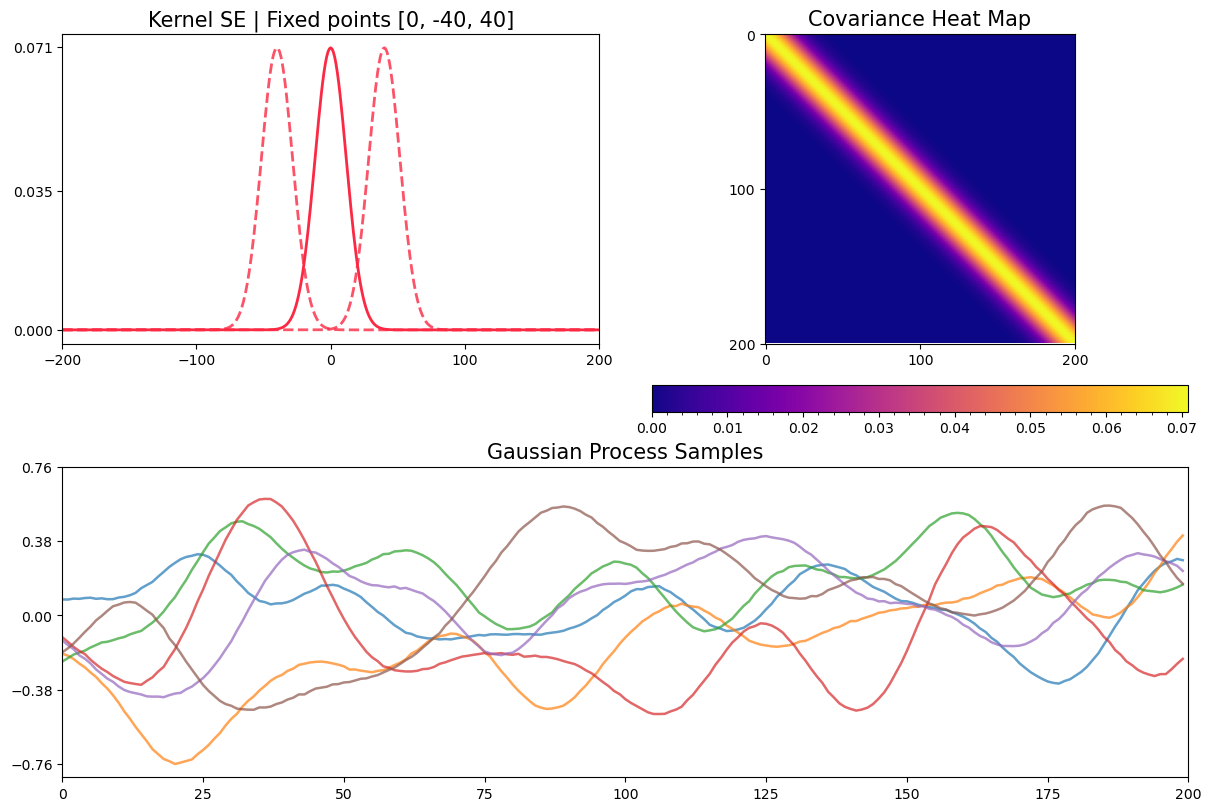
\includegraphics[scale=0.5]{k-SE}
	\caption{Representación gráfica del kernel exponencial cuadrático.}
\end{figure}

La construcción de \(k_{\mathrm{SE}}\) se puede realizar a partir de las funciones base
\begin{equation*}
	\phi_{c}(t) = \exp \left(-\frac{(t-c)^{2}}{2l^{2}}\right).
\end{equation*}
Si definimos la siguiente función de covarianza:
\[k(t_{p}, t_{q}) = \frac{\sigma_{p}^{2}}{N} \sum_{c=1}^{N} \phi_{c}(t_{p}) \phi_{c}(t_{q}),\]
y hacemos crecer la cantidad de puntos \(N\) a infinito, entonces se obtiene que
\begin{align*}
	\lim_{N \to \infty} \frac{\sigma_{p}^{2}}{N} \sum_{c=1}^{N} \phi_{c}(t_{p}) \phi_{c}(t_{q})	&= \sigma_{p}^{2} \int_{c_{\min}}^{c_{\max}} \phi_{c} (t_{p}) \phi_{c}(t_{q}) \dd{c} \\
																								&\to \sigma_{p}^{2} \int_{-\infty}^{\infty}\exp \left(-\frac{(t_{p} - c)^2}{2l^2}\right) \exp \left(-\frac{(t_{q} - c)^2}{2 l^2}\right) \dd{c} \\
	k(t_{p}, t_{q})																				&= \sqrt{\pi} l \sigma_{p}^{2} \exp \left(-\frac{(t_{p} - t_{q})^2}{2 (\sqrt{2} l)^2}\right).
\end{align*}
Como este kernel es isotrópico, entonces su densidad espectral también es isotrópica y gaussiana, como vimos en el primer capítulo.

\begin{proposition}
	La densidad espectral del kernel \(k_{\mathrm{SE}}(r)\) de parámetros \(h\) y \(l\) se escribe como
	\begin{equation*}
		S_{\mathrm{SE}}(s) = \frac{h}{\sqrt{2\pi} l} \exp \left(-2\pi^{2} l^{2} s^{2}\right).
	\end{equation*}
\end{proposition}

De forma análoga, si se tiene que una densidad espectral isotrópica tiene un dual de Fourier isotrópico, entonces ese dual es una función de covarianza. Esta densidad está en torno al origen, y si quisiéramos centrar la densidad espectral en torno a una frecuencia \(p\), debemos mantener la simetría en torno al origen para que sea válida. 

Veamos la siguiente construcción de densidad espectral en torno a la frecuencia \(p\), la cual genera el kernel conocido como Mixtura Espectral (\emph{Spectral Mixture} en inglés) que permite modelar comportamientos periódicos.

\begin{proposition}
	Consideremos la función gaussiana
	\[\phi_{p}(s) = \frac{1}{\sqrt{2\pi \sigma^2}} \exp \left(-\frac{(s - p)^{2}}{2\sigma^{2}}\right).\] Definiendo una densidad espectral de la forma \(S_{p}(s) = \frac{\phi_{p}(s) + \phi_{p}(-s)}{2}\), se tiene que su dual de Fourier es el kernel llamado \emph{Spectral Mixture}, un kernel estacionario de periodo \(p\), dado por
	\[k_{\mathrm{SM}}(r) = \exp \left(-2\pi^{2} \sigma^2 r^{2}\right) \cos(2\pi pr).\]
\end{proposition}

\begin{figure}[h]
	\centering
	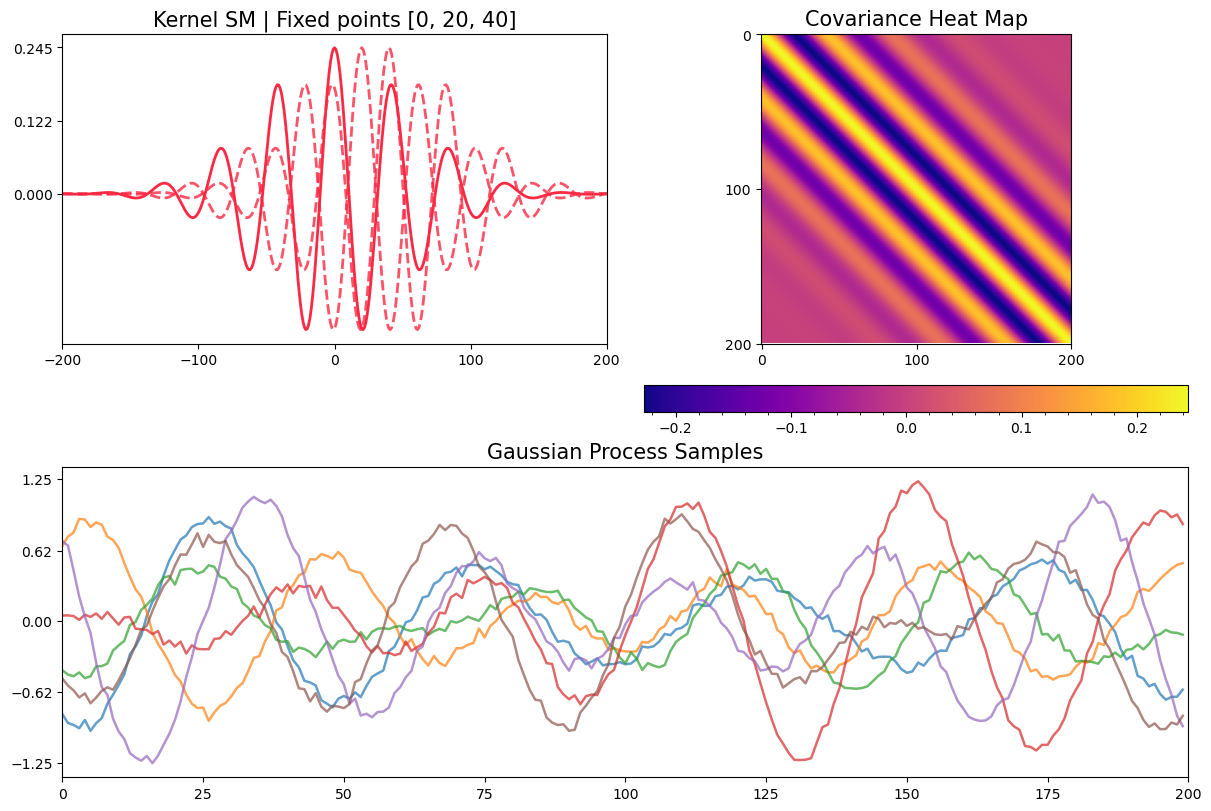
\includegraphics[scale=0.5]{k-SM}
	\caption{Representación gráfica del kernel spectral mixture.}
\end{figure}

La construcción anterior sigue siendo válida si consideramos varias frecuencias, incluso si consideramos el caso multidimensional no isotrópico.

\begin{proposition}
	Si se consideran \(N\) sumas de gaussianas multidimensional en \(\reals^{D}\)\cite{wilson2013gaussian}, entonces el kernel resultante es el \emph{Spectral Mixture} de \(N\) componentes.
	\begin{equation*}
		k(\bfr) = \sum_{q=1}^{N} \prod_{d=1}^{D} h_{q, d} \exp\left(-2\pi^{2} \sigma_{q, d}^{2} r_{d}\right) \cos(2\pi p_{q,d} r_{d}).
	\end{equation*}
\end{proposition}

Estos kernels permiten correlacionar puntos que estén a periodo \(\mu\) pero que no estén muy alejados, distancia controlada por el parámetro \(\sigma^2\). 

Un kernel que permite correlacionar los puntos que estén a periodo \(p\), de la misma forma independiente de la distancia de los puntos, es el kernel periódico definido como
\[ k_{\mathrm{Per}}(r) = h \exp \left(-\frac{2 \sen^{2}\left(\frac{\pi \vert r\vert}{p}\right)}{\ell^2}\right).\]

\begin{figure}[h]
	\centering
	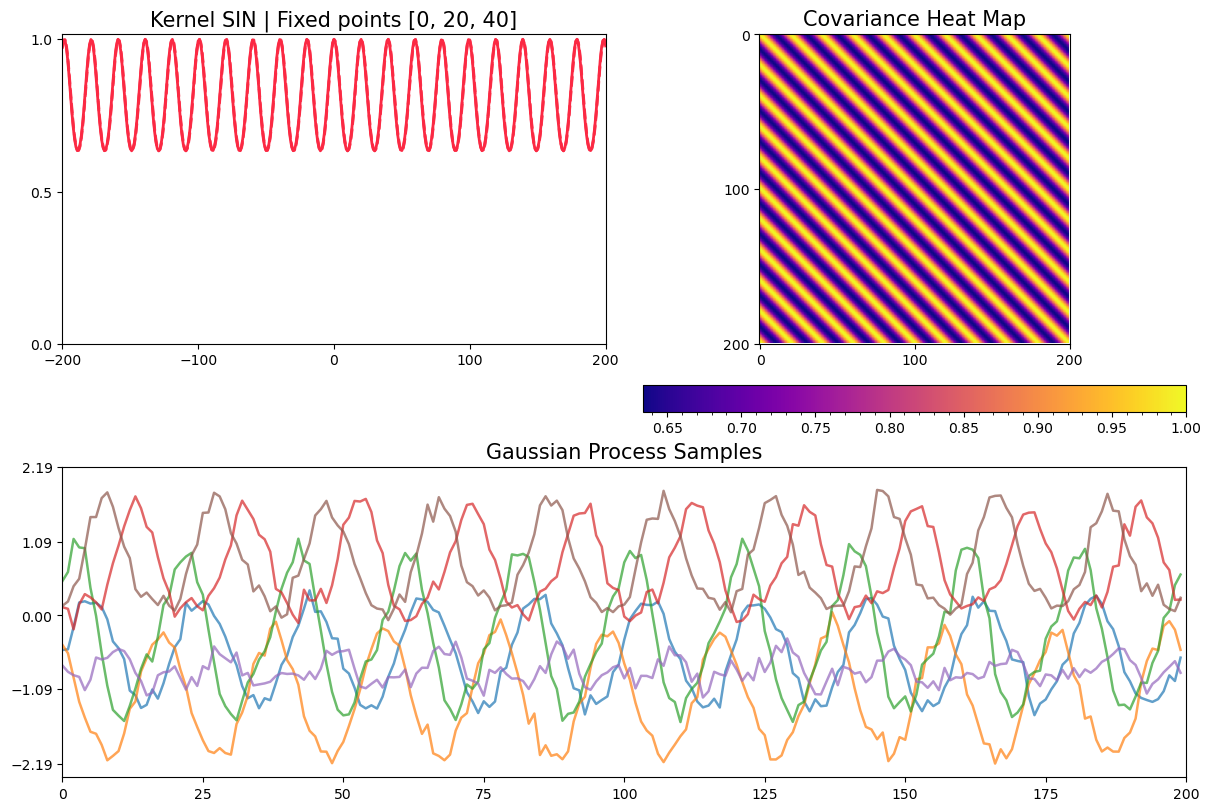
\includegraphics[scale=0.5]{k-SIN}
	\caption{Representación gráfica del kernel periódico.}
\end{figure}
El periodo \(p\) determina la distancia entre repetición de la función, y la escala \(\ell\) controla el nivel de correlación máxima.

Veamos algunos otros ejemplos de kernels estacionarios isotrópicos, destacando a la familia de kernels Matérn.
\begin{definition}
	Los kernels de Matérn depende de los parámetros \(v\) (la forma, \emph{shape} en inglés) y \(l\) (el largo, \emph{length} en inglés). Denotando \(\Gamma\) a la función gamma y \(K_{v}\) la función modificada de Bessel, estos kernels tienen la siguiente forma:
	\begin{equation*}
		k_{\mathrm{M}}(r) = h\frac{2^{1-v}}{\Gamma(v)} \left(\frac{\sqrt{2v} r}{l}\right)^{v} K_{v} \left(\frac{\sqrt{2v} r}{l}\right).
	\end{equation*}
\end{definition}

Dos de los casos más comunes son cuando \(v=3/2\) y \(v=5/2\):
\begin{align*}
	k_{v=3/2}(r)	&= h \left(1 + \frac{\sqrt{3} r}{l}\right) \exp \left(-\frac{\sqrt{3} r}{l}\right), \\
	k_{v=5/2}(r)	&= h \left(1 + \frac{\sqrt{5} r}{l} + \frac{5r^{2}}{3 l^{2}}\right) \exp \left(-\frac{\sqrt{5} r}{l}\right).
\end{align*}
En general, para todo parámetro \(v\) que cumpla \(v + \frac{1}{2} = p \in \naturals\), entonces la fórmula es un polinomio de grado \(p-1\) multiplicado por una exponencial. Esto indica a que mayor valor de \(v\), mayor es la suavidad del kernel. Más aún, cuando \(v \to \infty\), se tiene que este kernel converge a un exponencial cuadrático, es decir,
\begin{equation*}
	\lim_{n \to \infty} k_{v=n/2}(r) = k_{\mathrm{SE}}(r).
\end{equation*}

\begin{definition}
	Cuando \(v=1/2\), el kernel resultante es el exponencial, también conocido como el kernel de Laplace:
	\begin{equation*}
		k_{\mathrm{E}}(r) = h \exp \left(-\frac{r}{l}\right).
	\end{equation*}
\end{definition}

En dimensión \(1\), un proceso gaussiano con el kernel exponencial se llama el proceso de Ornstein-Uhlenbeck. 

\begin{figure}[h]
	\centering
	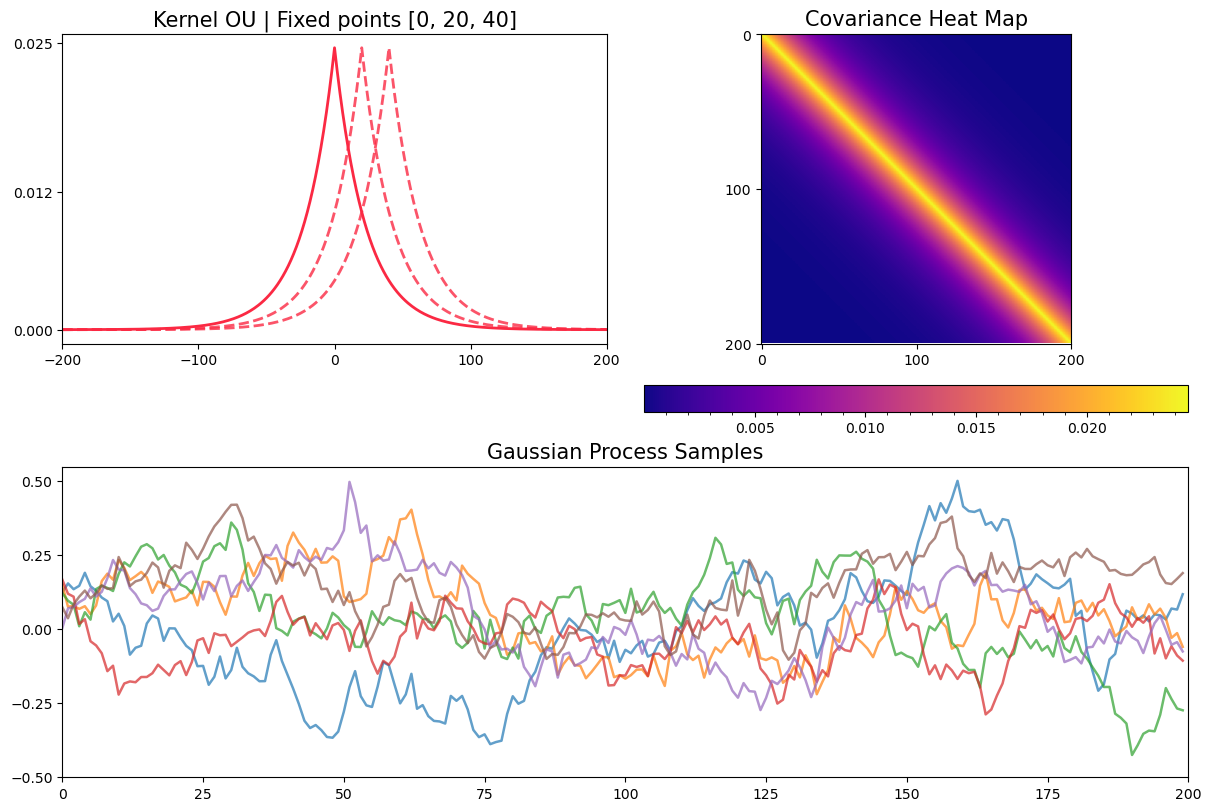
\includegraphics[scale=0.5]{k-OU}
	\caption{Representación gráfica del kernel de Laplace.}
\end{figure}

Veamos ahora una generalización del proceso exponencial y gaussiano.
\begin{definition}
	La familia \(\gamma\)-exponencial de kernels, para un valor de \(\gamma \in (0, 2]\), está dada por
	\begin{equation*}
		k_{\gamma}(r) = h \exp \left(-\left(\frac{r}{l}\right)^{\gamma}\right).
	\end{equation*}
\end{definition}

Ambas familia de kernels cumple una propiedades bastantes interesantes, ya que la suavidad de los procesos generados dependen de los parámetros de la familia del kernel. Ahora definiremos la noción de continuidad que utilizaremos para poder referirnos a la suavidad de un proceso.

\begin{definition}
	Diremos que el proceso \(\{x_{t}\}_{t \in \calI}\) es continuo en media cuadrática (\emph{mean-square} en inglés, y denotado MS-continuo) en un tiempo \(t\) si se cumple las siguientes dos condiciones:
	\begin{align*}
		\mean\left(\vert x_{t} \vert^{2}\right)							&< \infty, \\
		\lim_{s \to t} \mean\left(\vert x_{s} - x_{t}\vert^{2}\right)	&= 0.
	\end{align*}
\end{definition}

\begin{definition}
	Diremos que el proceso es diferenciable en media cuadrática (denotado MS-diferenciable) en un tiempo \(t\) si su derivada en dicho tiempo existe y se cumple que
	\begin{align*}
		\lim_{\triangle t \to 0} \mean\left( \left\vert \dv{x_{t}}{t} \right\vert^{2}\right)	&< \infty, \\
		\lim_{\triangle t \to 0} \mean\left( \left\vert \frac{x_{t + \triangle t} - x_{t}}{\triangle t} - \dv{x_{t}}{t} \right\vert^{2} \right) &= 0.
	\end{align*}

	De forma recursiva, diremos que un proceso es \(k\)-diferenciable en media cuadrática en un tiempo \(t\) si su \(k\)-ésima derivada en dicho tiempo existe, es continua en media cuadrática y cumple que:
	\begin{equation*}
	\lim_{\triangle t \to 0} \mean \left( \left\vert \frac{\dv[k-1]{x_{t + \triangle t}}{t} - \dv[k-1]{x_t}{t}}{\triangle t} - \dv[k]{x_{t}}{t} \right\vert^2\right) = 0.
	\end{equation*}
\end{definition}

Ahora que tenemos definida la noción de continuidad y diferenciabilidad en media cuadrática, veamos la suavidad de los diferentes procesos generados.
\begin{proposition}
	El proceso de Ornstein-Uhlenbeck es MS-continuo pero no es MS-dife\-ren\-ciable. El proceso con kernel \(\gamma\)-exponencial no es MS-diferenciable salvo cuando \(\gamma = 2\), en cuyo caso es infinitamente MS-diferenciable. El proceso de Matérn con parámetro \(v\) es \(\lceil v-1 \rceil\) veces MS-diferenciable.
\end{proposition}

De las familias \(\gamma\)-exponencial y Matérn con parámetro \(v\), el kernel SE es el único que cumple la propiedad de ser infinitamente MS-diferenciable. Existen otros kernels con esta propiedad, entre los cuales destaca el kernel conocido racional cuadrático. Veamos a continuación su definición y cómo se puede interpretar.

\begin{definition}
	El kernel racional cuadrático (\emph{rational quadratic} en inglés, denotado RQ) de parámetros \(\alpha > 0\) (la forma, \emph{shape} en inglés) y \(l > 0\) (el largo, \emph{length} en inglés) se define como
	\[ k_{\mathrm{RQ}}(r) = h \left(1 + \frac{r^2}{2\alpha l^2}\right)^{-\alpha}.\]
\end{definition}

\begin{figure}[h]
	\centering
	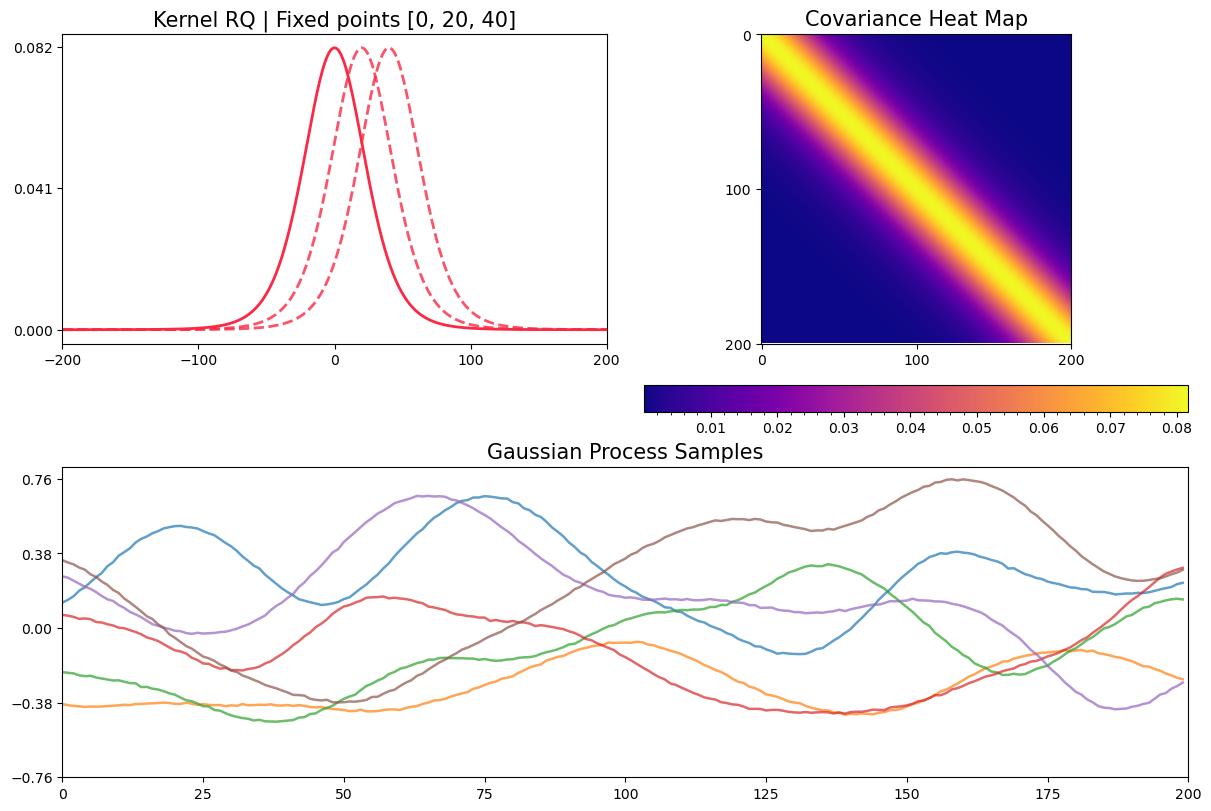
\includegraphics[scale=0.5]{k-RQ}
\end{figure}

El kernel RQ puede verse como una suma infinita de kernels SE con diferentes escalas \(l\), donde el parámetro \(\alpha\) determina el peso relativo, o proporción, entre variaciones de alta o baja escala. Si parametrizamos como \(\tau = l^{-2}\) con una distribución gamma \(p (\tau \mid \alpha, \beta) \propto \tau^{\alpha - 1} \exp (-\alpha \tau / \beta )\), entonces integrando un kernel SE con respecto \(\tau\) se tiene que
\begin{align*}
	k_{\mathrm{RQ}}(r)	&= \int p(\tau \mid \alpha, \beta) k_{\mathrm{SE}}(r \mid \tau) \dd{\tau} \\
						&\propto \int \tau^{\alpha-1} \exp \left(-\alpha \frac{\tau}{\beta} \right) \exp \left(-r^{2} \frac{\tau}{2}\right) \dd{\tau} \\
						&\propto \left(1 + \frac{r^{2}}{2\alpha l^{2}}\right)^{-\alpha},
\end{align*}
con \(\beta = l^{-2}\). Con esta construcción, y usando el hecho de que el operador derivada conmuta con la integral, es directo ver que este kernel hereda la suavidad del kernel SE. Además, a medida de que \(\alpha\) tiende a infinito, el kernel RQ converge a un kernel SE:
\begin{equation*}
	\lim_{\alpha \to \infty} \sigma^2 \left(1 + \frac{r^{2}}{2\alpha l^{2}}\right)^{-\alpha} = \sigma^2 \exp\left(\frac{r^{2}}{2 \ell^{2}}\right).
\end{equation*}

\begin{proposition}
	El proceso generado con un kernel RQ es infinitamente MS-diferencia\-ble, para cualquier \(\alpha > 0\).
\end{proposition}

Todos los kernels mostrados hasta ahora son isotrópicos. Sin embargo, todos los kernels isotrópicos \(k_{r}\) puedes convertirse a anisotrópicos reemplazando \(r^{2}\) por una función que depende de una matriz semidefinida positiva \(M\) tal que
\begin{equation*}
	k_{r} \left(r^{2}(t, \bar{t})\right) = k_{r}\left((t-\bar{t})^{\top} M (t-\bar{t})\right).
\end{equation*}
Si \(M\) es una matriz diagonal, entonces el kernel escala cada dimensión de forma independiente. La transformación más general es de la siguiente forma:

\begin{proposition}
	Dado un kernel isotrópico \(k_{r}\), se define el kernel
	\begin{align*}
		k_{M} (t, \bar{t})	&= k_{r}\left((t - \bar{t})^{\top} M (t-\bar{t}) \right), \\
		M					&= \Lambda \Lambda^{\top} + \Psi,
	\end{align*}
	donde \(\Lambda\) es una matriz de dimensión \(D \times k\), sus columnas definen \(k\) direcciones de gran relevancia, y \(\Psi\) es una matriz diagonal positiva que captura la relevancia de cada dimensión. El kernel \(k_{M}\) es un kernel estacionario anisotrópico.
\end{proposition}

\subsection{Kernels de Producto Interno}

Todos los kernels estudiados hasta ahora cumplen la propiedad de ser estacionarios. En muchos casos, el proceso que se desea estimar no cumple con el supuesto de estacionalidad, al tener una componente no estacionaria. Una forma de modelar dicha componente es con una función de media. Otro enfoque es considerar kernels no estacionarios, donde la familia más destacada son aquellos con forma de producto punto.

El kernel de producto punto más simple es el kernel lineal, definido como
\[ k_{\mathrm{Lin}} (t, \bar{t}) = \sigma_{0}^{2} + \langle t, \bar{t}\rangle.\]

\begin{figure}[h]
	\centering
	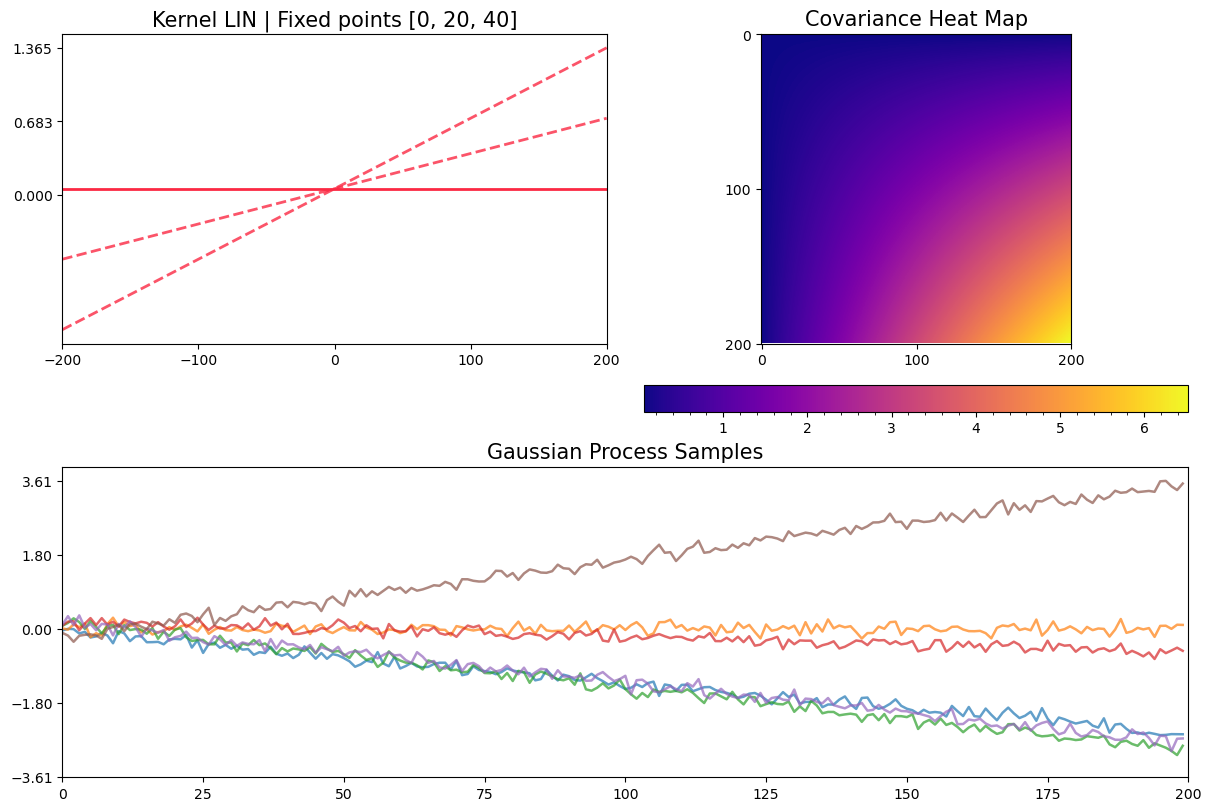
\includegraphics[scale=0.5]{k-LIN}
	\caption{Representación gráfica del kernel lineal.}
\end{figure}

Este kernel que permite modelar dependencias lineales con respecto a las variables de entrada, y se le conoce como Regresiones Lineales Bayesianas. Si \(\sigma_{0}^{2} = 0,\) entonces se dice kernel lineal homogéneo. Como es un producto punto, es posible incluir una matriz definida positiva \(\Sigma_{p}\) entre las componentes de \(t\), de la misma forma que se construyen los kernels anisotrópicos, quedando el kernel lineal generalizado como
\begin{align*}
	k_{\mathrm{Lin}} (t, \bar{t})	&= \sigma_{0}^{2} + t^{\top} \Sigma_{p} \bar{t},\\
	\Sigma_{p}						&= \Lambda \Lambda^{\top} + \Psi.
\end{align*}
Con el kernel lineal es posible incluir dependencias lineales. Es natural pensar en kernels que nos permitan modelar otro tipo de dependencias, tales como cuadráticas o polinomiales en general. Para esto, definamos el kernel polinomial de grado \(n\).

\begin{definition}
	El kernel polinomial \(k_{n} (t, \bar{t}) = \left(\sigma_{0}^{2} + t^{\top} \Sigma_{p} \bar{t}\right)^{n}\) es una función de covarianza válida para \(n \in \naturals^+\).
\end{definition}

Para ver que este kernel es una función de covarianza válida, basta con poder expresarlo en forma de producto punto. Por simplicidad, consideremos el caso isométrico homogéneo:
\begin{align*}
	k_{n}(t, \bar{t})	&= \langle x, \bar{t} \rangle^{n} \\
						&= \left(\sum_{d=1}^{D} t_{d} \bar{t}_{d}\right)^{n}\\
						&= \prod_{i=1}^{n} \left(\sum_{d=1}^{D} t_{d} \bar{t}_{d}\right) \\
						&= \sum_{d_{1}=1}^{D} \dotsb \sum_{d_{n}=1}^{D} \left(\prod_{i=1}^{n} t_{d_{i}}\right) \left(\prod_{i=1}^{n} \bar{t}_{d_{i}}\right)\\
						&= \langle \bfphi(t), \bfphi(\bar{t}) \rangle.
\end{align*}
A priori, se pensaría que la suma tiene \(D^{n}\) términos, pero como el orden de las multiplicaciones \(t_{d_{1}}, \dotsc, t_{d_{n}}\) conmuta, es posible reducir el número de términos definiendo un vector \(\bfm = (m_1, \dotsc, m_D)\), donde la componente \(m_{d}\) especifica el número de veces que la componente \(t_{d}\) aparece en el monomio bajo la restricción de que \(\sum_{i=1}^{D} m_{i} = n\). La función \(\bfphi(t)\) está definida por componentes indexadas por los vectores \(\bfm\), donde la función característica \(\phi_{\bfm}(t)\) es proporcional al monomio \(t_{1}^{m_{1}}, \dotsc, t_{D}^{m_{D}}\) y degenerada en \(\frac{n!}{m_{1}! \dotsb m_{D}!}\):
\begin{equation*}
	\phi_{\bfm}(t) = \sqrt{\frac{n!}{m_{1}!...m_{D}!}} t_{1}^{m_{1}} \dotsb t_{D}^{m_{D}}.
\end{equation*}
Esto implica que las funciones generadas son combinaciones lineales de los monomios de todos los órdenes, produciendo cualquier polinomio homogéneo de orden \(n\). Si al espacio de entrada le agregamos una coordenada constante \(t_{0} = 1\), entonces es posible reproducir cualquier polinomio de orden hasta \(n\). De forma equivalente, en vez de agregar una coordenada constante basta con sumar una constante \(\sigma_{0}^{2}\) antes de elevar a \(n\). El kernel polinomial cumple la propiedad que la varianza crece rápidamente a medida que \(\vert x \vert\) crece, pero si los datos están normalizados entonces este kernel entrega buenos resultados.

Siguiendo este mismo enfoque, podemos construir la función \(\bfphi\) con cualquier base finita de funciones, generando funciones utilizando dicha base. La construcción más simple es considerar un hiperparámetro por cada elemento de la base, con el fin de determinar cuales funciones son relevantes.
\begin{definition}
	Dada una base de funciones \(\Phi = \{\phi_{i}\}_{i=1}^{N}\), el kernel máquina de relevancia vectorial (\emph{relevance vector machine} en inglés, denotado RVM) es de la forma
	\begin{equation*}
		k_{\mathrm{RVM}}(t, \bar{t}) = \sum_{j=1}^{N} \frac{1}{\alpha_{j}} \phi_{j}(t) \phi_{j}(\bar{t}).
	\end{equation*}
\end{definition}

\begin{proposition}
	El kernel RVM es una función de covarianza degenerada (el espacio de características es finito-dimensional).
\end{proposition}

A medida de que el término \(\alpha_{j}\) se acerque a infinito, la componente \(\phi_{j}\) tiene menos relevancia en la covarianza del proceso, mientras que los términos cercanos a cero explican la mayor parte de la varianza. A su vez, podemos generalizar la expresión anterior utilizando la matriz definida positiva \(\Sigma_{p} = \Lambda \Lambda^{\top} + \Psi\), produciendo el kernel de forma
\begin{align*}
	k_{\Sigma_{p}}(t, \bar{t})	&= \bfphi(t)^{\top} \Sigma_{p} \bfphi(\bar{t}) \\
								&= \sum_{i=1}^{N} \sum_{j=1}^{N} \sigma_{ij} \phi_{i}(t) \phi_{j}(\bar{t}).
\end{align*}

\subsection{Otros Kernels de Covarianza}
Existen funciones de covarianza que no son estacionarias y tampoco tienen forma de producto punto. Un ejemplo clásico es el kernel que produce el movimiento browniano o el kernel producto.

\begin{proposition}
	El proceso de Wiener con función de covarianza \(k(t, \bar{t}) = \min \{x, \bar{t}\}\) es un proceso no estacionario.
\end{proposition}

\begin{figure}[h]
	\centering
	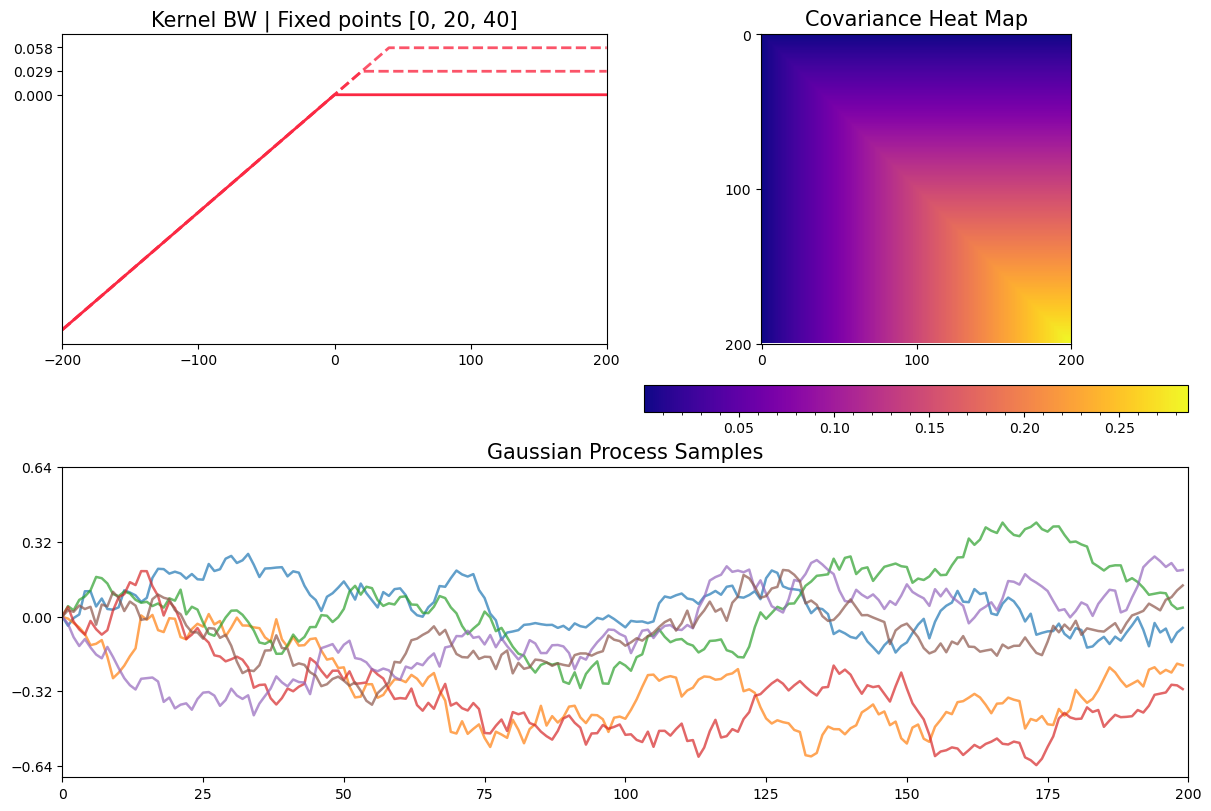
\includegraphics[scale=0.5]{k-BW}
	\caption{Representación gráfica del kernel browniano.}
\end{figure}

\begin{proposition}
	El proceso de ruido blanco (\emph{white noise} en inglés) con función de covarianza \(k(t, \bar{t}) = \delta_{x, \bar{t}}\) es un proceso no estacionario.
\end{proposition}

Existen muchos otros kernels válidos que pueden construirse utilizando funciones no lineales, las cuales se aplican después de operar \(t\) con \(\bar{t}\). Un ejemplo es el kernel red neuronal (\emph{neural network kernel} en inglés) definido como
\begin{equation*}
	k_{\mathrm{NN}}(t, \bar{t}) = \frac{2}{\pi} \arcsin \left(\frac{2x^{\top} \Sigma_{p}\bar{t}}{\left(1 + 2x^{\top} \Sigma_{p} \bar{t}\right) \left(1 + 2x^{\top} \Sigma_{p} \bar{t}\right)}\right).
\end{equation*}
Este kernel es válido y es no estacionario. Sin embargo, no todas las funciones generan kernels válidos, por ejemplo el kernel sigmoide
\begin{equation*}
	k(t, \bar{t}) = \tanh(a + b \langle x, \bar{t}\rangle),
\end{equation*}
no es definida positiva para ningún valor de \(a\) y \(b\). Otro kernel no estacionario válido es el kernel de base gaussiana, definido como
\begin{align*}
	k_{\mathrm{GB}}(t, \bar{t})	&= \frac{1}{(2\pi \sigma_u^2)^{d/2}} \int \exp\left(-\frac{\vert x-u \vert^2}{2\sigma_g^2} - \frac{\vert \bar{t}-u \vert^2}{2\sigma_g^2} -\frac{\langle u, u\rangle}{2\sigma_u^2}\right) \dd{u} \\
								&= \left(\frac{\sigma_e}{\sigma_u}\right)^d \exp\left(-\frac{\langle x, x \rangle}{2 \sigma_m^2}\right) \exp\left(-\frac{\vert x-\bar{t}\vert^2}{2\sigma_s^2}\right) \exp\left(-\frac{\langle \bar{t}, \bar{t}\rangle}{2\sigma_m^2}\right), \\
\end{align*}
donde
\begin{align*}
	\frac{1}{\sigma_{e}^{2}}	&=\frac{2}{\sigma_{g}^{2}}+\frac{1}{\sigma_{u}^{2}},\\
	\sigma_{s}^{2}				&= 2\sigma_{g}^{2}+\frac{\sigma_{g}^{4}}{\sigma_{u}^{2}},\\
	\sigma_{m}^{2}				&= 2\sigma_{u}^{2}+\sigma_{g}^{2}.
\end{align*}
Este kernel converge al exponencial cuadrático cuando \(\sigma_{u}^{2} \to \infty\), por lo que podemos interpretar que el término \(\sigma_{u}^{2}\) controla el grado de no estacionalidad.

Otra forma de crear kernels es a partir de kernels estacionarios. Si \(u\) es una función de características no lineal y \(k_{u}(u, \bar{u})\) es un kernel estacionario en \(u\), entonces
\begin{equation*}
	k_{t, u}(t, \bar{t}) = k_{u}(u(t), u(\bar{t})),
\end{equation*}
es un kernel para \(t\). Consideremos el caso en que \(u(t) = (\cos(t), \sen(t))\) y \(k_{u}\) es SE, entonces
\begin{equation*}
	k_{t, u}(t, \bar{t}) = \exp \left(-\frac{2\sen^{2}\left(\frac{x-\bar{t}}{2}\right)}{\ell^{2}}\right)
\end{equation*}
coincide con el kernel periódico. Es posible construir kernels de forma más complejas pero que conserven la propiedad de definido positivo. Un ejemplo es el kernel de la forma
\begin{equation*}
	k(t, \bar{t}) = \prod_{d=1}^{D} \left(\frac{2\ell_{d}(t) \ell_{d}(\bar{t})}{\ell_{d}^{2}(t) + \ell_{d}^{2}(\bar{t})}\right) \exp\left(-\sum_{d=1}^{D} \frac{(t_{d}-\bar{t}_{d})^{2}}{\ell_{d}^{2}(t) + \ell_{d}^{2}(\bar{t})}\right),
\end{equation*}
donde cada \(\ell_{d}\) es una función positiva de \(t\), es una función de covarianza que para todo \(t\) cumple \(k(t, t) = 1\). Otro ejemplo es considerar un kernel \(k_{S}\) estacionario e isotrópico, y una función \(\Sigma\) a valores matriciales de dimensión \(D \times D\) definida positiva. Luego el kernel
\begin{equation*}
	k_{\mathrm{NS}}(t, \bar{t}) = \frac{2^{\frac{D}{2}} \vert \Sigma(t) \vert^{\frac{1}{4}} \vert \Sigma(\bar{t}) \vert^{\frac{1}{4}}}{\vert \Sigma(t) + \Sigma(\bar{t}) \vert^{\frac{1}{2}}} k_{S}\left(\left((t-\bar{t})^{\top} \left(\frac{\Sigma(t) + \Sigma(\bar{t})}{2}\right) (t-\bar{t})\right)^{\frac{1}{2}}\right),
\end{equation*}
es una función de covarianza no estacionaria.


\section{Composición de Kernels}

En la sección anterior revisamos las familias de kernels más comunes. Es posible construir nuevos kernels a partir de un kernel base y funciones auxiliares. Veamos a continuación algunas formas de construir kernels que mantienen la propiedad de ser definido positivo.

\subsection{Composición con funciones auxiliares}

La forma más simple de construir kernels es partir desde un único kernel base, para luego componerlo con alguna función auxiliar. Veamos a continuación las composiciones válidas.

\begin{proposition}
	Sea \(k\) un kernel definido positivo, \(n \in \naturals\), \(u\) una función unaria y \(h\) una función binaria (ambas funciones arbitrarias). Entonces las siguientes construcciones producen kernels válidos:
	\begin{itemize}
		\item Potencia: \(\tilde{k}(t, \bar{t}) = k^{n}(t, \bar{t})\).
		\item Normalización: \(\tilde{k}(t, \bar{t}) = \frac{k(t, \bar{t})}{\sqrt{k(t, t)} \sqrt{k(\bar{t}, \bar{t})}}\).
		\item Escalamiento: \(\tilde{k}(t, \bar{t}) = u(t) k(t, \bar{t}) u(\bar{t})\).
		\item Composición: \(\tilde{k}(t, \bar{t}) = k(u(t), u(\bar{t}))\).
		\item Convolución: \(\tilde{k}(t, \bar{t}) = \int \int h(t, s) k(s, \bar{s}) h(\bar{t}, \bar{s}) \dd{s} \dd{\bar{s}}\).
		\item Reflexión: \(\tilde{k}(t, \bar{t}) = k(t, \bar{t}) + k(-t, \bar{t}) + k(t, -\bar{t}) + k(-t, -\bar{t})\).
	\end{itemize}
\end{proposition}

Cada una de estas construcciones produce funciones con alguna propiedad. Por ejemplo, si \(f(t) \sim \GP(0, k)\), entonces el escalamiento produce funciones de la forma \(f(t) u(t)\), la composición funciones de la forma \(f(u(t))\), la potencia funciones de la forma \(f^{n}(t)\), la convolución funciones de la forma \(\tilde{f}(t) = \int f(s) h(s, t) \dd{s}\) y la reflexión permite generar funciones simétricas \(\tilde{f}(t) = \tilde{f}(-t) = f(t) + f(-t)\).

\subsection{Composición entre Kernels}

Además de manipular un único kernel para obtener otro diferente, también es posible componer kernels entre sí, manteniendo la propiedad de ser definido positivo \cite{12} \cite{13}. Veamos las operaciones de
composición válidas entre kernels.

\begin{proposition}
	Sean \(k_{1}\) y \(k_{2}\) dos kernels de covarianza. Entonces las siguientes composiciones producen kernels válidos.
	\begin{itemize}
		\item Suma: \(k(t, \bar{t}) = k_{1}(t, \bar{t}) + k_{2}(t, \bar{t})\).
		\item Producto: \(k(t, \bar{t}) = k_{1}(t, \bar{t}) k_{2}(t, \bar{t})\).
		\item Punto de Cambio (\emph{Changepoint} en inglés):
		\[k(t, \bar{t}) = \sigma(t) k_{1}(t, \bar{t}) \sigma(\bar{t}) + (1-\sigma(t)) k_{2}(t, \bar{t}) (1 - \sigma(\bar{t})),\]
		donde \(\sigma(t) = (1 + e^{-x})^{-1}\) o alguna función creciente de \(0\) a \(1\).
	\end{itemize}
\end{proposition}

Cada una de estas composiciones produce un efecto distinto. Una forma de interpretar la composición de kernels es utilizando su representación de producto punto en el espacio de componentes. Consideremos \(k_{1}(t, \bar{t}) = \bfphi_{1}(t)^{\top} \bfphi_{1}(\bar{t})\) y \(k_{2}(t, \bar{t}) = \bfphi_{2}(t)^{\top} \bfphi_{2}(\bar{t})\). Luego la suma se puede expresar como
\begin{align*}
	k_{1}(t, \bar{t}) + k_{2}(t, \bar{t})	&= \bfphi_{1}(t)^{\top} \bfphi_{1}(\bar{t}) + \bfphi_{2}(t)^{\top} \bfphi_{2}(\bar{t}) \\
											&= \begin{bmatrix} \bfphi_{1}\left(t\right) \\ \bfphi_{2}\left(t\right) \end{bmatrix}^{\top} \begin{bmatrix} \bfphi_{1}(\bar{t}) \\ \bfphi_{2}(\bar{t}) \end{bmatrix},
\end{align*}
la cual coincide con concatenar las dimensiones del espacio de características. A su vez, la multiplicación se puede expresar como
\begin{align*}
	k_{1}(t, \bar{t}) k_{2}(t, \bar{t})	&= \left( \bfphi_{1}^{\top}(t) \bfphi_{1}(\bar{t}) \right) \left(\bfphi_{2}(t)^{\top} \bfphi_{2}(\bar{t}) \right) \\
										&= \left(\sum_{i} \phi_{1}^{(i)}(t) \phi_{1}^{(i)}(\bar{t})\right) \left(\sum_{j} \phi_{2}^{(j)}(t) \phi_{2}^{(j)}(\bar{t})\right) \\
										&= \sum_{i, j} \left(\phi_{1}^{(i)}(t) \phi_{2}^{(i)}(\bar{t})\right) \left(\phi_{1}^{(j)}(t) \phi_{2}^{(j)}(\bar{t}) \right),
\end{align*}
la cual coincide con multiplicar las dimensiones del espacio de características.

Otra interpretación posible surge desde el espacio de las funciones generadas por cada proceso. La suma de kernels se interpreta como la superposición de procesos independientes, cada uno correspondiente a uno de los kernels en la suma. Esto se deduce del siguiente resultado.
\begin{figure}[h]
	\centering
	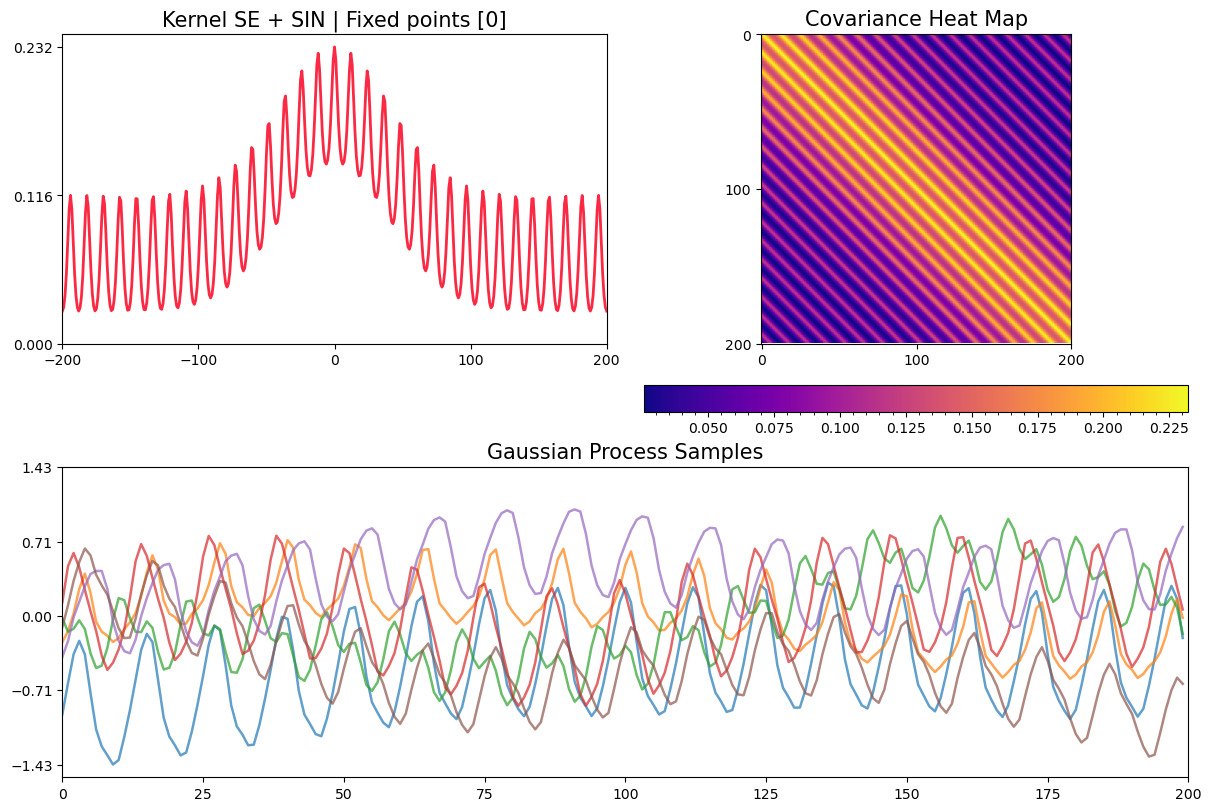
\includegraphics[scale=0.5]{k-SE+SEN}
	\caption{Representación gráfica de la suma de kernels SE + SEN.}
\end{figure}

\begin{proposition}
	Sean \(f_{1} \sim \GP(\mu_{1}, k_{1})\) y \(f_{2} \sim \GP(\mu_{2}, k_{2})\) dos GP independientes. Entonces la suma es un GP de la forma
	\begin{equation*}
		f = f_{1} + f_{2} \sim \GP(\mu_{1} + \mu_{2}, k_{1} + k_{2}).
	\end{equation*}
\end{proposition}

El resultado permite poder descomponer la función \(f\) en las componentes \(f_{1}\) y \(f_{2}\). Sean \(T, \bff\) los datos observados. Si suponemos que \(\bff = \bff_{1} + \bff_{2}\), entonces podemos estimar \(\bff_{1}\) (y \(\bff_{2}\)) utilizando la distribución posterior de \(f_{1}\) (y \(f_{2}\)) dado \(f\):
\begin{equation*}
	\bar{\bff}_{1} \mid \bff, T, \bar{t} \sim \calN\left(\bar{\mu}_{1} + \bar{\bfk}_{1}^{\top} (\mathbf{K}_{1} + \mathbf{K}_{2})^{-1} (\bff - \mu_{1} - \mu_{2}), \bar{\mathbf{K}}_{1} - \bar{\bfk}_{1}^{\top} (\mathbf{K}_{1}
	+ \mathbf{K}_{2})^{-1} \bar{\bfk}_{1}\right)
\end{equation*}
donde \(\mathbf{K}_{i} = k_{i}(T, T)\), \(\bar{\mathbf{K}}_{1} = k_{1}(\bar{t}, \bar{t})\) y \(\bar{\bfk}_{1} = k_{1}(\bar{t}, T)\). Si se modela \(f\) como \(\GP(0, k_{1} + \dotsb + k_{n})\), entonces es posible descomponer \(f\) en la suma \(f_{1} + \dotsb + f_{n}\), donde sus respectivas posteriores tienen la siguiente forma:
\begin{align*}
	f_{d}(\bar{t})	&\sim \calN\left(\mu_{d}, \sigma_{d}^{2}\right), \text{ para } d=1, \dotsc, n,\\
	\mu_{d}			&= k_{d}(\bar{t}, T) \left[ \sum_{i=1}^{n} k_{i}(T, T) \right]^{-1} f(t), \\
	\sigma_{d}^{2}	&= k_{d}(\bar{t}, \bar{t}) - k_{d}(\bar{t}, T) \left[ \sum_{i=1}^{n} k_{i}(T, T) \right]^{-1} k_{d}(T, \bar{t}).
\end{align*}

Por otro lado, el producto de kernels es considerado como una operación \textsc{AND}, ya que para que \(t\) y \(\bar{t}\) estén correlacionados deben estarlo bajo el criterio de ambos kernels \(k_{1}\) y \(k_{2}\). Los efectos que se logran al multiplicar kernels dependen del kernel escogido. Veamos los siguientes efectos:

\begin{itemize}
	\item Sea \(k\) un kernel que tiene una estructura de correlación global (como el caso lineal). Al multiplicarlo por un kernel SE se remueven las correlaciones lejanas, ya que decrece monótamente a medida de que la distancia crece.
	\item Sea \(k\) un kernel que genera las funciones \(f(t) \sim \GP(0, k)\). Al multiplicar dicho kernel con un kernel LIN las funciones generadas corresponden a las originales multiplicadas por un término en \(t\), es decir, \(t f(t) \sim \GP(0, k k_{\mathrm{Lin}})\).
	\item Sea \(k\) un kernel que genera las funciones \(f(t) \sim \GP(0, k)\). Al multiplicar dicho kernel con un kernel PER las funciones generadas corresponden a las originales multiplicadas por una función periódica independiente, es decir, \(f(t) f_{\mathrm{Per}}(t) \sim \GP(0, k k_{\mathrm{Per}})\), donde \(f_{\mathrm{Per}} \sim \GP(0, k_{\mathrm{Per}})\).
\end{itemize}

\begin{figure}[h]
	\centering
	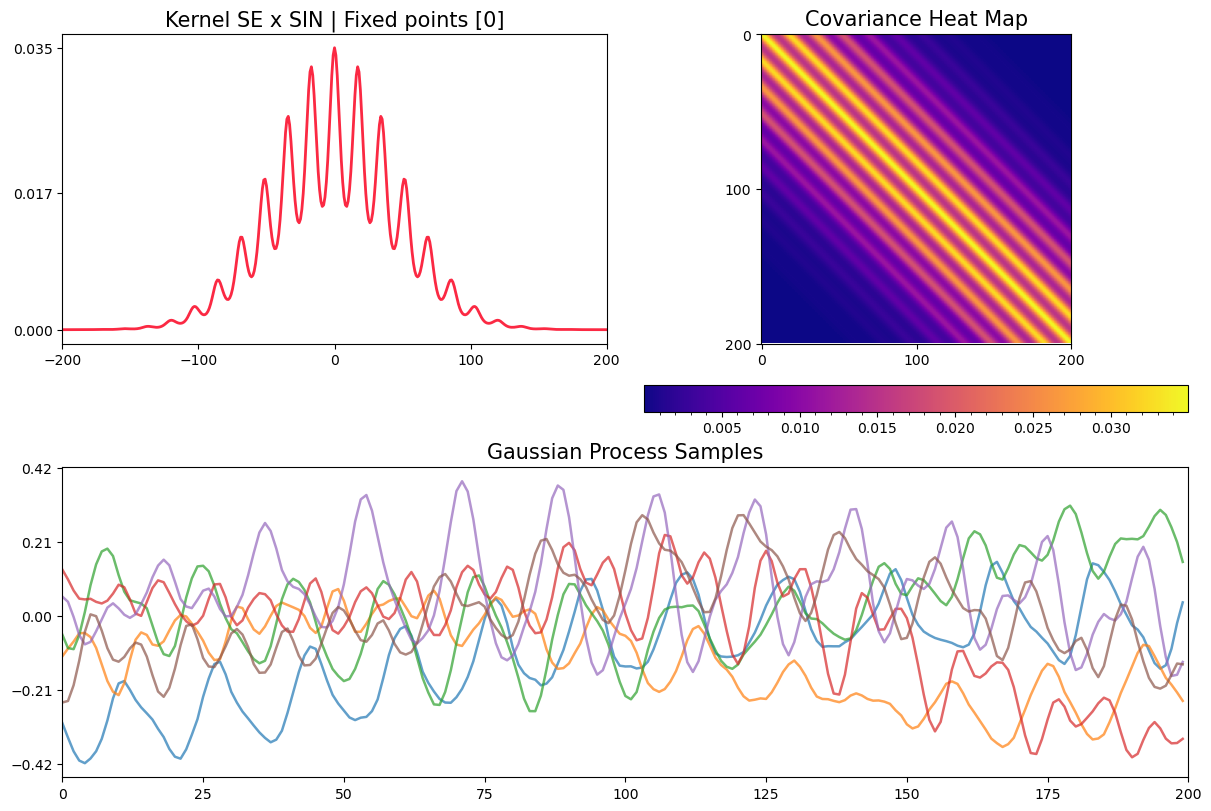
\includegraphics[scale=0.5]{k-SE-SEN}
	\caption{Representación gráfica de la multiplicación de kernels SE * SEN.}
\end{figure}

La composición del tipo \emph{changepoint} entre los kernels \(k_{1}\) y \(k_{2}\) entrega el kernel \(\CP(k_{1}, k_{2})\), que se mueve de un kernel al otro dependiendo una función \(\sigma\), que indica cuál de los dos se activa. La idea de utilizar la función logística es porque así el cambio se produce de forma suave.

Dado que el kernel resultante es válido, uno puede volver a aplicar un \emph{changepoint} con otra función, definiendo así ventanas para cada uno de los kernels de la composición. Esto generaliza la operación compuesta de \emph{change-window}, donde se reemplaza \(\sigma\) por la multiplicación de una sigmoide creciente con otra decreciente. Veamos algunos de los kernels compuestos más utilizados, donde el tipo de funciones que generan tienen ciertas propiedades interesantes y que tienen una interpretación útil.
\begin{enumerate}
	\item El kernel cuadrático (\emph{Quadratic Kernel} en inglés) tiene la forma
	\begin{align*}
		k_{\mathrm{Qua}}(t, \bar{t})	&= k_{\mathrm{Lin}}(t, \bar{t}) k_{\mathrm{Lin}}(t, \bar{t}) \\
										&= \sigma_{0}^{2} + \sigma_{1}^{2} x^\top \bar{t} + \sigma_{2}^{2}\left[x^\top \bar{t}\right]^{2}.
	\end{align*}
	Este kernel permite modelar dependencias cuadráticas y lineales entre el espacio de entrada y la salida.
	\item El kernel localmente periódico (\emph{Locally Periodic Kernel} en inglés) tiene la forma
	\begin{align*}
		k_{\mathrm{LocalPer}}(t, \bar{t})	&= k_{\mathrm{SE}}(t, \bar{t}) k_{\mathrm{Per}}(t, \bar{t}) \\
											&= \sigma^2 \exp \left(-\frac{(t - \bar{t})^{2}}{2\ell_{\mathrm{SE}}^2}\right) \exp \left(-\frac{2 \sen^{2} \left(\frac{\pi \vert x - \bar{t}\vert}{p}\right)}{\ell_{\mathrm{Per}}^2}\right).
	\end{align*}
	Este kernel permite modelar funciones que son localmente periódicas, pero que la forma puede ir variando lentamente.
	\item El kernel multiperiódico (\emph{Multi Periodic Kernel} en inglés), también conocido como la descomposición generalizada de Fourier (\emph{generalized Fourier decomposition} en inglés), se basa en sumar varios kernels periódicos
	\begin{align*}
		k_{\mathrm{GFD}}(t, \bar{t})	&= \sum_{i=1}^{n} k_{\mathrm{Per}}^{(i)}(t, \bar{t}) \\
										&= \sum_{i=1}^{n} \sigma_{i}^{2} \exp \left(-\frac{2\sen^{2}\left(\frac{\pi \vert x - \bar{t} \vert}{p_i}\right)}{\ell_{i}^{2}}\right).
	\end{align*}
	Este kernel se interpreta como la descomposición de la función en \(n\) frecuencias diferentes.
	\item El kernel lineal periódico (\emph{Linear Periodic Kernel} en inglés) tiene la forma
	\begin{align*}
		k_{\mathrm{LinPer}}(t, \bar{t})	&= k_{\mathrm{Lin}}(t, \bar{t}) k_{\mathrm{Per}}(t, \bar{t}) \\
										&= (\sigma_{b}^{2} + \sigma_{v}^{2} x^\top \bar{t}) \exp \left(-\frac{2\sen^{2} \left(\frac{\pi \vert x - \bar{t} \vert}{p}\right)}{\ell^{2}}\right).
	\end{align*}
	Este kernel permite modelar funciones periódicas que tienen una amplitud incremental a medida que se aleja de un centro.
	\item El kernel lineal más periódico (\emph{Linear Plus Periodic Kernel} en inglés) tiene la forma
	\begin{align*}
		k_{\mathrm{Lin+Per}}(t, \bar{t})	&= k_{\mathrm{Lin}}(t, \bar{t}) + k_{\mathrm{Per}}(t, \bar{t}) \\
											&= \sigma_{b}^{2} + \sigma_{v}^{2} x^\top \bar{t} + \sigma_{0}^{2} \exp \left(-\frac{2\sen^{2}\left(\frac{\pi \vert x - \bar{t}\vert}{p}\right)}{\ell^{2}}\right).
	\end{align*}
	Esta combinación simple se puede interpretar como la clásica descomposición de los efectos de tendencia y periodicidad. En general, se puede cambiar la componente de tendencia por otro kernel más ad hoc, y sumar más de un kernel periódico, para descomponer en efectos de periodo corto y de periodo largo.
\end{enumerate}

\subsection{Composición Multidimensional}

La composición no debe ser necesariamente con kernels del mismo espacio de entrada. Veamos a continuación una proposición que generaliza esto.

\begin{proposition}
	Sea \(k_{1}\) un kernel en \(\calT_{1}\) y \(k_{2}\) un kernel en \(\calT_{2}\). Si definimos el espacio \(\calT = \calT_{1} \times \calT_{2}\) con \(t = (t_{1}, t_{2})\), entonces los siguientes kernels son funciones de covarianza en \(\calT\):
	\begin{itemize}
		\item Suma Directa: \(k(t, \bar{t}) = k_{1}(t_{1}, \bar{t}_{1}) + k_{2}(t_{2}, \bar{t}_{2})\). Cuando se suman kernels que sólo dependen de una sola dimensión de la variable de entrada, el espacio de funciones corresponde a la suma de cada espacio de funciones, es decir, si \(f_{1} \sim \GP(0, k_{1}) \) y \(f_{2} \sim \GP(0, k_{2})\), entonces \(k_{1} + k_{2}\) genera funciones de la forma
		\[f(t_{1}, t_{2}) = f_{1}(t_{1}) + f_{2}(t_{2}) \sim \GP(0, k_{1} + k_{2}).\]
		
		\item Producto Tensor: \(k(t, \bar{t}) = k_{1}(t_{1}, \bar{t}_{1}) k_{2}(t_{2}, \bar{t}_{2})\). Cuando se multiplican kernels que sólo dependen de una sola dimensión de la variable de entrada, los puntos deben ser similares en todas las dimensiones para que tengan alta correlación. Esta operación es similar a un \textsc{AND}.
	\end{itemize}
\end{proposition}

Para ver la diferencia entre la suma directa y el producto tensor entre dos kernels, consideremos el caso que la función tenga una estructura aditiva, por ejemplo \(f(t_{1}, t_{2}) = \sen(t_{1}) + \sen(t_{2})\). En este caso, el kernel aditivo extrapola la función en puntos lejanos de los datos de entrenamiento, mientras que el kernel multiplicativo permite interpolar la función entre los datos de entrenamiento, pero al extrapolar se revierte a la media.

Con estas composiciones entre dimensiones, podemos formar diferentes kernels de \(D\) dimensiones, y darle una cierta interpretación a los coeficientes correspondientes a cada dimensión. Veamos un par de ejemplos de kernels
compuestos multidimensionales.
\begin{enumerate}
	\item El modelo aditivo generalizado (\emph{Generalized Additive Model} en inglés) tiene la forma
	\begin{equation*}
		k_{\mathrm{GAM}}(t, \bar{t}) = \sum_{d=1}^{D} \sigma_{d}^{2} \exp\left(-w_{d}^{2} (t_{d} - \bar{t}_{d})^{2}\right).
	\end{equation*}
	En este kernel se interpreta el parámetro \(\sigma_{d}^{2}\) como la magnitud de la componente en la covarianza, y \(w_{i}^{2}\) indica la escala de la componente \(t_{i}\).
	\item El kernel automático de determinación de relevancia (\emph{Automatic Relevance Determination Kernel} en inglés) tiene la forma
	\begin{equation*}
		k_{\mathrm{ARD}}(t, \bar{t}) = \sigma^2 \exp \left(-\sum_{d=1}^{D} w_{d}^{2} (t_{d} - \bar{t}_{d})^{2}\right).
	\end{equation*}
	En este kernel se interpreta el parámetro \(w_{i}^{2}\) como la relevancia de la componente \(t_{i}\) en la covarianza.
	\item El kernel aditivo de orden \(n\)-ésimo (\emph{nth Order Additive Kernel} en inglés) tiene la forma
	\begin{equation*}
		k_{\mathrm{addn}}(t, \bar{t}) = \sigma^2 \sum_{1\leq i_{1} < \dotsb <i_{n} \leq D} \prod_{d=1}^{D} k_{i_{d}}\left(t_{i_{d}}, \bar{t}_{i_{d}}\right).
	\end{equation*}
	Esta familia de kernels \cite{30} es una generalización del kernel ARD, en donde se consideran los subconjuntos de variables de cardinalidad \(n \leq D\), y en cada dimensión \(d\) se tiene un kernel \(k_{d}\) asociado.
	\item El kernel reflexivo multidimensional (\emph{Reflexive Multidimensional Kernel} en inglés) nace a partir de un kernel \(k_{2D}\) de dos dimensiones. Si lo componemos consigo mismo, cambiando el orden en una componente
	\begin{equation*}
		k_{S2D}([t, s], [\bar{t}, \bar{s}]) = k_{2D}([t, s], [\bar{t}, \bar{s}]) + k_{2D}([s, t], [\bar{t}, \bar{s}]),
	\end{equation*}
	este nuevo kernel modela funciones de dos dimensiones que son simétricas. Es decir, si \(f \sim \GP(0, k_{S2D})\) entonces
	\begin{equation*}
		f(t, s) = f(s, t).
	\end{equation*}
	Para extender a más dimensiones basta con incluir más permutaciones del orden de las variables.
	\item El kernel de codificación de baja dimensionalidad (\emph{Low Dimensional Encode Kernel} en inglés) supone que el espacio de entrada \(\calT\) tiene dimensión alta. En muchos casos se da que la función buscada es de baja dimensión, es decir, que pertenece a un subespacio de dimensión menor al generado con el kernel \(k\). En ese caso, es posible bajar la dimensión a través de una matriz \(A\) de menor rango de forma que
	\begin{equation*}
		k_{\mathrm{low}}(t, \bar{t}) = k(At, A\bar{t}).
	\end{equation*}
	Si sumamos el kernel de menor rango con el kernel original, es posible obtener un efecto de variabilidad local adicional:
	\begin{equation*}
		k_{\mathrm{low+}}(t, \bar{t}) = k(At, A\bar{t}) + k(t, \bar{t}).
	\end{equation*}
\end{enumerate}


\comment{parrafo: concluir capitulo, mencionar otros temas, mencionar papers y otros avances en el tema}